
\chapter{Neural Network Components: Layers}
\label{Layers}


\begin{figure}[!ht]
    \centering
    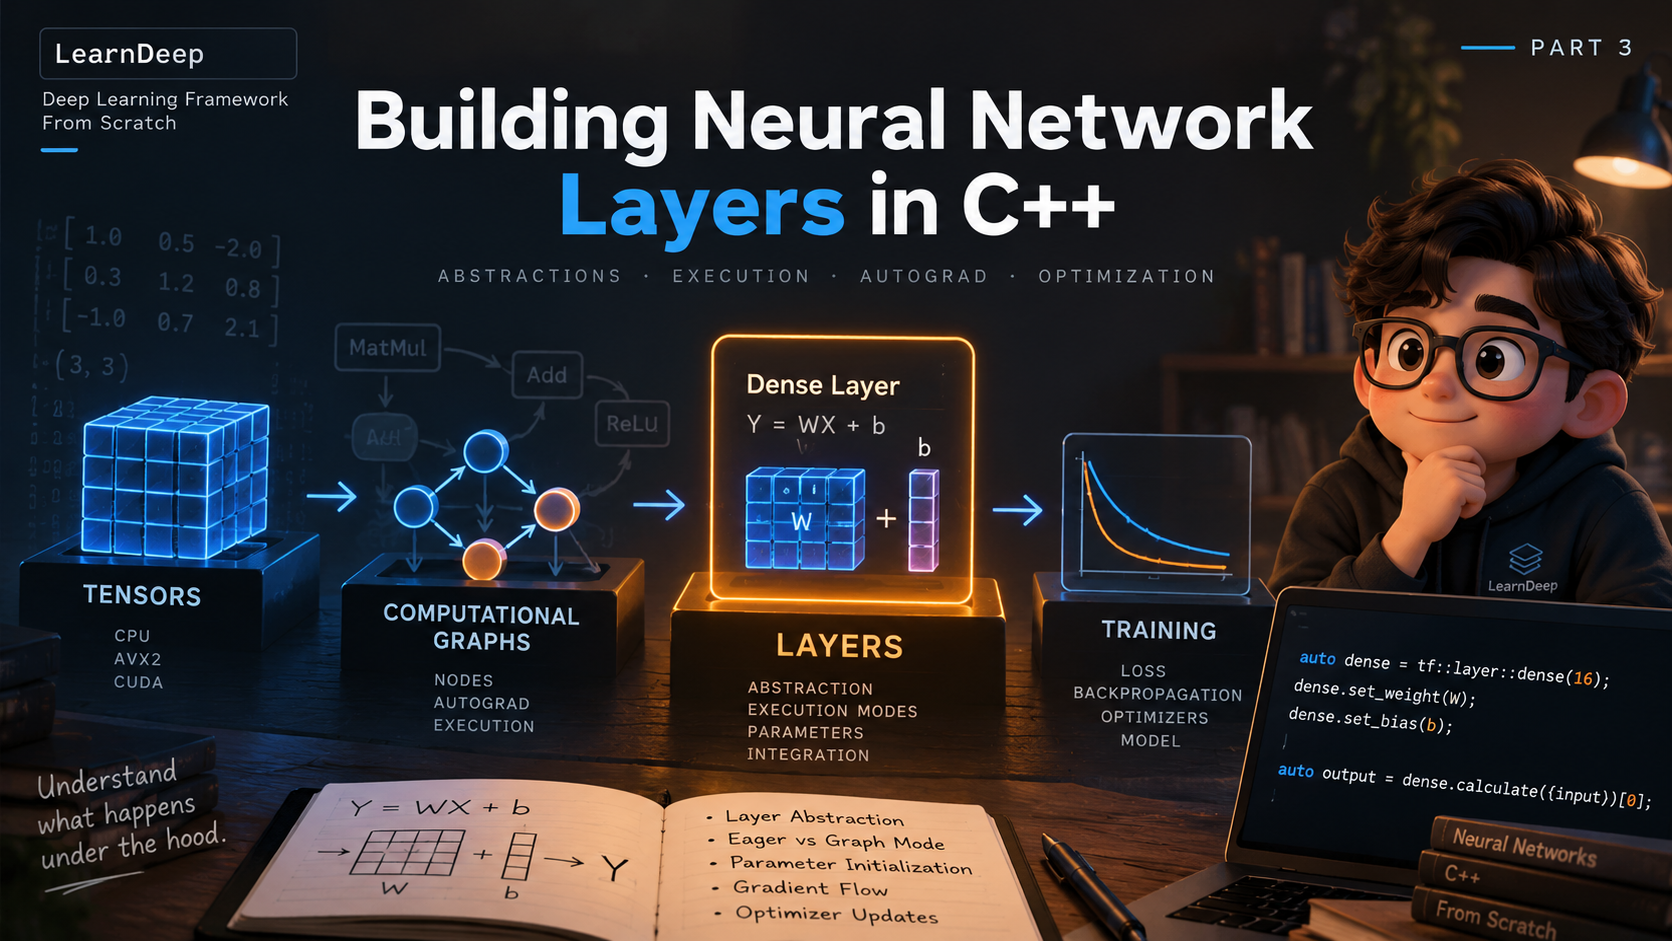
\includegraphics[width=\textwidth]{../../images/06_Building Neural Network Layers in C++.png
    }
\end{figure}

\section{Layer}
A layer is a high-level abstraction that encapsulates a
sequence of mathematical operations into a reusable
component. It allows us to construct complex neural
network architectures without explicitly writing
every underlying operation or manually defining the
backward graph for each layer.

This abstraction separates model architecture from the
mathematical details of individual operations. As a
result, we can modify the architecture and its
hyperparameters while relying on the framework to
handle the underlying computations and automatic
differentiation.

Let's now examine how layers are implemented in this framework.

The Layer class is an abstract base class that defines
the common interface for derived layers. Each concrete
layer implements the required functions:

the layer class is a abstruct class i.e can't be instantiated
then later layers are inheriting and overriding the functions
like
\begin{itemize}
    \item calculate: Calculates the forward pass only in eager
    mode
    \item forward: Constructs the layer's computation in the
    current graph context for graph-mode execution.
    \item backward: Retrieves the gradients required by the
    layer's parameters and registers the corresponding optimizer
    update operations. It does not explicitly construct the
    backward graph for the layer's mathematical operations;
    those gradients are handled by the autograd system.
    \item basic constructor and destructors and some axulary
    functions to intercept the parameters or hyperparameters.
\end{itemize}

Let's see it in practice

\begin{lstlisting}[
    caption={Creating layer class},
    label={lst:layer abstruct class}
]
class Layer {
public:
    virtual ~Layer() = default;

    virtual std::vector<tf::tensor>
    calculate(std::vector<tf::tensor> inputs) = 0;
    virtual std::vector<tf::tensor*>
    forward(std::vector<tf::tensor> inputs) = 0;
    virtual void backward() = 0;
};
\end{lstlisting}

Now lets take a look at each layer and how they're constructed

\section{Layer: Dense}

Mathematically Dense layer is very simple, it does matmul bias
add, which is

$
Y = X@W + b
$

\begin{itemize}
    \item X: input temsor of rank 2. axis-1 is feature
    axis-2 is batch or sample size.
    \item W: is weights tensor of rank 2 axis-1 is Dense
    unit/no or neuron axis-2 is no of incoming features.
    \item b: is a vector or matrix of rank 1. axis-1 is
    no of dense unit/ no of neuron.
    \item Y: output tensor of rank 2. axis-1 is no of
    feature and axis-2 is batch or sample size.
\end{itemize}

The idea behind Dense layer is do a linear transformation on
input with weights tensor and add bias to it.

If we wanted to implemente a dense layer without any layer
abstruction it would look something like


\begin{lstlisting}[
    caption={Dense Function},
    label={lst:Dense Function}
]
#include <tensor.h>

tf::tensor X, W, B, Y;

X.tf_create(18, 512); // no_of_input_feature(18), and sample_size(512)
W.tf_create(16, 18);  // dense_unit(16), and no_of_incoming_feature(18)
B.tf_create(18); // dense_unit(16);

Y = X.matmul(W).add(B);
\end{lstlisting}

First of all we can we that but if we think from bigger
perspective then it would be very clear that. This approch
is not that easy to scale. If we get to the training phase
then we need to mannually handle gradients and update them.
So that is the reason behind abstruction.

No Lets take a look at how to properly make the abstruction

\subsection{Dense: Constructor}

\begin{lstlisting}[
    caption={Dense constuctor and basic structure},
    label={lst:Dense constructor and basic structure}
]
// file dense.hpp
#include <layer.hpp>

Class Dense : protected Layer{
    Dense(unsigned unit): dense_unit(unit){}

    std::vector<tf::tensor *>& operator(std::vector<tf::tensor> input_tensors);
    std::vector<tf::tensor> calculate(std::vactor<tf::tensor> inputs) override;
    std::vector<tf::tensor *>& forward(std::vector<tf::tensor> inputs, unsigned const batch_size) override;
    std::vector<tf::tensor *>& backward(Optimizer *const optimizer) override;
    ...
    // few other internal methods/functions
    ...
}
\end{lstlisting}

simple easy peasy no rocket science. constructor
is expecting the no of neuron for this layer.
and assigning the vaue to its internal variable
and few other internal flags, weights, bias initialization
methods are set. Which is not shown here.

\subsection{Dense: Overloaded () operator}


\begin{lstlisting}[
    caption={Dense () overloaad},
    label={lst:Dense () overloaad}
]

// file dense.cpp
#include "dense.hpp"

const std::vector<tf::tensor *> &
Dense::operator()(std::vector<const tf::tensor> input_tensors){
    if(input_tensor.size() == 1){
        weights.tf_create();
        bias.tf_create();
        layer_outputs.push_back(tf::tensor(tf_float64));
    } else {
        // throw error, Dense layer expects only one input tensor
    }

}
\end{lstlisting}

The overloaded operator() provides a convenient
interface for connecting layers. During this
stage, the layer prepares its parameters and
output handles as required by the framework.

The initialization is lazy because the layer
may not have enough information to initialize
all its internal state when the constructor
is called. The first build or forward operation
provides the necessary context, such as the
input shape and batch size.

The output handle is particularly important:
it allows subsequent layers to reference the
output of this layer without manually
connecting every underlying mathematical
operation.

Why use vectors of tensors instead of a single
tensor? Although a Dense layer accepts one input
tensor and produces one output tensor, the base
interface supports layers that may consume
multiple inputs or produce multiple outputs.
This keeps the layer interface general without
forcing every layer to use the same input/output
cardinality.


\subsection{Dense: forward() backward() calculate()}

\begin{lstlisting}[
    caption={Dense calculate},
    label={lst:Dense calculate}
]

// file dense.cpp
#include "dense.hpp"

const std::vector<tf::tensor *> &
Dense::forward(std:;vector<const tf::tensor *> &inpyt, unsigned batch_size){

      this->weight.reshape(arr);
      this->training_weight.tf_create(arr, tf_float64);
      this->grad_weight.tf_create(arr, tf_float64);

      ...
      // initialize bias
      // initialize outputs
      ...

      training_output.push_back(training_input.matmul(training_weights).add(training_bias));

      return training_ouput;

}



const std::vector<tf::tensor *> &
Dense::calculate(std:;vector<const tf::tensor *> &inpyt, unsigned batch_size){
initializeParameters();
std::vector<tf::tensor> output;

output.emplace_back(inputs[0].matmul(weights).add(bias));

return output;
}

Dense::backward(Optimizer *optimizer){

  if (!this->isGradRecorded) {
    Graph *g = GraphManager::instance().getCurrentGraph();
    graph_weight = g->getGradTensor(training_weight);
    grad_bias =  g->getGradTensor(training_bias);
    grad_input = g->getGradTensor(training_inputs[0]);
    grad_output = g->getGradTensor(training_output[0]);

    optimizer->createParameterUpdateGraph(training_weight, updated_weight, grad_weight);
    optimizer->createParameterUpdateGraph(training_bias, updated_bias, grad_bias);

    this->isGradRecorded = true;
  }
}
\end{lstlisting}

Lets discuss one at a time:

\subsubsection{forward() }

This function implements the graph-mode forward
path and is primarily invoked during model
training through fit().

At this stage, the framework has access to the
execution context and the relevant input shapes.
The layer can initialize its parameters, prepare
the required tensors, and construct the
computation using the framework's primitive
operations.

The graph context is managed by the model's
training procedure, so the layer does not
need to create a separate graph context for
itself.

The important distinction is that forward()
constructs the computation graph; it does not
necessarily evaluate the tensor operations
immediately.

\subsubsection{calculate()}
This function implements the eager-mode
forward path and is primarily used by
predict() when immediate inference is
required.

Unlike graph construction, eager execution
evaluates the underlying operations as they
are invoked and returns the resulting
output tensors.

\subsubsection{backward()}
It retrieves the gradients associated with
the weights, biases, inputs, and outputs
from the current graph context, as required
by the implementation. It then registers
the parameter update operations with the
optimizer.

The gradients of the layer's mathematical
operations are computed by the autograd
system. The layer's backward() method
does not manually derive those gradients;
instead, it exposes the relevant gradient
tensors and prepares the optimizer update path.

The isGradRecorded flag prevents these
registrations from being repeated unnecessarily
within the intended graph lifecycle.

\subsection{Dense in practice}

\begin{lstlisting}[
    caption={Dense in practice},
    label={lst:Dense in practice}
]
// file dense_test_01.cpp
#include <tensor.h>

void main(){
    tf::tensor inputs, W, B, ouputs;

    inputs.tf_create(tf_float64, 19, 1000);
    W.tf_create(tf_float64, 16, 19); // tensor to seed weight
    B.tf_create(tf_tf_float64, 16);  // tensor to seed bias

    input.tensor_of(-2.0, 3.0);
    W.tensor_of(-1.0, 1.0);
    B.tensor_of(0.0, 0.0);

    auto dense = tf::layer::dense(16); // 16 is dense unit a.k.a no of neurons
    dense.set_weight(W);
    dense.set_bias(B);

    output = dense.calculate({inputs})[0]; // output holds the output from dense layer

}
\end{lstlisting}

\subsubsection{Dense Training}

backward(), is already covered so, we know
how it is done in code but let's touch upon
mathematical construct of Dense backward

Weight updation

\[ \bar{W} \leftarrow W - \nu * {\delta{W}} \]
\[ {\delta{W}} = ZX^T \]

Bias updation
\[ \bar{B} \leftarrow B - \nu * {\delta{B}} \]
\[ {\delta{W}} = X \]

Gradient propagation

\[ {\delta{X}} = W^TZ \]

The input gradient is propagated to the preceding
layer; it is not updated using the learning rate.
The optimizer updates trainable parameters, while
autograd propagates gradients through the
computational graph.


Where,
\[ Z \text{ is incoming grad} \]
\[ X \text{ is input} \]


